\documentclass{ltjbook}
\usepackage{docmute} 
\usepackage{../../myStyle} 

\begin{document}
\VerbatimFootnotes
\chapter{Bayesian Inference and Decision Making}
\label{m27_bayesian3}
So far, we have talked about Bayesian methods. How do you feel about them?
Compared to the traditional frequentist approach, it is difficult to definitively say which is better when considering the use of probability models, the fact that results are also obtained as probability distributions, and the different way of thinking about probabilities. It may be difficult to decide as there are some differences. For example, when considering why psychology needs statistics, it may be challenging to tackle but we cannot ignore it by simply saying "I don't like either method."

By the way, there was a discussion about using the traditional method of statistical hypothesis testing to determine the presence or absence of effects. How would this work in Bayesian methods? That is the theme of this article.

\section{Bayesian Methods and Null Hypothesis Testing}
Let's take a moment to review the concept of \keytermE{hypothesis testing}.

Using a \keytermE{factor design}{要因計画}{よういんけいかく} approach in research, individual differences and errors are taken into account by creating two groups (or more) based on data that may contain such differences, and then averaging them to offset individual effects. An operation is then performed on one group to determine the causal effect, and the group average is analyzed to view the typical effect. The factor design breaks down the sources of influence into various factors and interactions using a \keytermE{linear model}{線形モデル}{せんけいもでる} that decomposes the overall variance into element-wise summation. This allows for determining the magnitude of the effects.

"I am a translator. Without modifying the TeX code, please translate this Japanese text into English:

'However, since the magnitude of the sample effect has its limits, we want to extend this to the world of the population. That's where the field of \keytermE{inferential statistics} comes in. We estimate the position of the mean and the magnitude of the effect based on the sample.'"
In hypothesis testing, we are provided with criteria for determining whether an effect was present or absent. Two hypotheses/models are set up: one stating that there is no effect, and the other stating that there is some effect. We then consider which model is better.
In this process, we start by assuming the "null hypothesis" that there is no effect, and proceed with calculations based on this assumption to determine how much the actual value deviates from the model. We consider how unlikely the actual value is, using the distribution of the ratio of variances (F-distribution) or the difference in means of two groups (t-distribution) to assess how much greater the effect is compared to the intensity. If the result is smaller than the predetermined criterion, i.e. the "significance level," it means that something rare has occurred in reality, and we conclude that the null hypothesis was wrong. If the null hypothesis is proven wrong, we conclude that "there is a difference." We can use this conclusion to either think "we need to investigate further," or judge that "saying there is no difference means there is a difference." In the latter case, we need to be careful because there is a risk of making a "type 1 error" by falsely claiming there is a difference when there is none, or "type 2 error" by falsely claiming there is no difference when there is one. Instead of hastily making a decision on whether there is a difference or not, we should quantitatively assess the magnitude of the effect using an indicator called "effect size," and report it accordingly. Additionally, if we repeat judgments too many times, we may lose control over type 1 errors, so we must proceed with caution and analyze the main effects first before conducting post-hoc tests.

Phew! Summarizing what I’ve been explaining in multiple frames, it would read something like this in a single paragraph. It's quite a hassle! Particularly, you might get confused at points where I say "I can't claim there is no difference," or the probability of saying that there is no difference when there actually is. At least I always get nervous while teaching this, wondering if I might make a mistake. Why is such a complicated approach appreciated? The reason is that this way of thinking does not require the idea of a prior probability distribution, and if we assume that whatever data we obtain seems to be derived from a normal distribution, we can proceed with this testing procedure mechanically.

The discussion on hypothesis testing originated from agriculture. The idea of dividing sections and comparing the effects came from experiments on the growth of crops conducted in agricultural testing facilities. Once the format for this analysis was developed, it could be applied to psychology as well. Although humans are not products harvested in agricultural testing facilities, their various characteristics are likely to follow a normal distribution, making it possible to use this method. This applies not only to psychology, but also to biology, economics, physics, sociology, and various other fields. As long as there are ideas such as data distribution and normal distribution of errors, the method can be applied. Moreover, the arduous calculations involved in this analytical procedure! Mathematical derivations are especially difficult, dealing with things such as t-distributions and F-distributions. However, since the calculation format is established, simply inputting it into R's function will provide results. Even without thinking about complex matters, results can be obtained. This is why the hypothesis testing is so valuable. The format being established makes it possible to apply the method to various fields, and statistical packages that implement the calculation format are available. Therefore, even those of us who are not good at mathematics can obtain the power of statistics. However, this has become a problem. That is, people use it without fully understanding it, and only look at the results. It's like trying to drive a car even though you don't have a license, simply because you stepped on the accelerator and the car started moving. If you do something like this in the real world, it's a very dangerous thing to do. However, statistics is a difficult subject, too specialized, and there is no other choice but to entrust some of it to machines or previous advancements. After all, more people use automatic transmission cars than manual ones, and an amateur expert would not have enough specialized knowledge to repair the computer control part of an automatic transmission vehicle. It's too much to say that you can't drive without understanding everything. Therefore, we must acquire a basic level of knowledge that allows us to obtain a license and be mindful of not using it for evil purposes or misusing it. Furthermore, just as a license needs to be renewed, we should not neglect our studies of statistics. If we find that we cannot master new techniques, we should also consider returning our licenses and not driving.

As specialists in psychology, we do not have a good understanding of statistics and can only approach it from the perspective of a user of tools. I believe this is true. However, at the same time, if we claim to specialize in psychology, we must take more responsibility for interpreting and understanding the results. As I mentioned earlier, while it is certainly one way to determine the criteria for judging whether a difference can be said to exist through mechanical means when the null hypothesis is rejected, we must first consider carefully how much of a difference is of substantive significance and what constitutes a difference. In the end, hypothesis testing is just one way of determining the results of interval estimates, and we must consider the difference between the estimated mean, its interval, effect size, and the confidence interval for the effect size itself.

It is important to note that, under the conventional frequency-based approach, the estimated mean is treated as a constant value. The \textbf{confidence interval} is a number that represents the \textbf{proportion} of the estimated mean that is contained within that interval, and does not provide information on the range of the interval itself despite being called an interval. On the other hand, the \textbf{credible interval} derived from the posterior distribution of the mean value, for instance, the mean value of each group, obtained through Bayesian methods, represents the \textbf{range of probable values} for the stochastically distributed mean value, and is the actual information on the width of the interval. In Bayesian methods, the interval estimation of the estimated mean represents the region of belief, from lower to upper limits, or the range of possible values, and is not a matter of accuracy.

Moreover, the Bayesian approach requires a prior distribution, which can lead to criticisms such as "it is inappropriate to manipulate data based on subjective beliefs about whether there will be differences before conducting an analysis".
However, on the other hand, there is also a discussion about whether it is really a good idea to have no premises at all \citep{Maeda2017}.

For example, let's consider the story of flipping a coin and getting "heads" 7 times out of 24 flips. We want to test whether this is a fair coin or not using a null hypothesis test. The null hypothesis is that the coin has no bias towards "heads" or "tails". The alternative hypothesis is that there is some bias present. Although the data falls just short of half (12 flips), when we actually perform the null hypothesis test, we cannot reject the null hypothesis\footnote{To test whether a frequency distribution like 7 "heads" and 14 "tails" is biased, we use a $\chi^2$ test. In R, if we enter \texttt{chisq.test(c(7,14))}, we get the answer $\chi^2(1)=2.33, p=0.1266$.}. In other words, the result of 7 "heads" out of 24 is a result that is likely to occur more than 5\% of the time, and is not particularly surprising.

But what if instead of a coin, it was a nail? You would toss the nail and consider it heads if the pointed end landed on the ground and stood up. If not, it would be tails. Let's say you tried this 24 times and the nail stood up 7 times. Why is that? Isn't it strange? Unusual? Incredible?

Even in situations like this, the null hypothesis cannot be rejected. The fact that there were 7 heads out of 24 flips is a fact, and the conclusion is that "it's not impossible, these things happen." We think "there's no way that a thrown nail would land on its head," because we have a strong belief that it's impossible. This belief is backed by physical laws and is thoroughly convincing. However, even such beliefs should not be ignored under the principle of "we must not have any preconceptions," and if we take the attitude that "we must not have any preconceptions, and that the data revealed is all there is," then we can only support the answer that there is no bias. Is this what defines a scientist?

The null hypothesis test does not only rely on prior beliefs, but also does not refer to the generation process or mechanism behind the data. On the other hand, when conducting Bayesian estimation, it's necessary to specify the prior distribution and the likelihood. The prior distribution reflects the researcher's prior knowledge, and the likelihood represents the mechanism behind the data. Therefore, Bayesian statistics, which clearly records this information, can be considered a more open approach.


\section{Judging by Intervals}
The main reason why conducting a hypothesis test can be cumbersome is that it involves probabilistic judgments. It can be confusing because one must consider the probability of making an incorrect judgement.
In contrast, the \keytermE{Bayesian approach}{ベイズ法} considers "the world I believe in" rather than considering "the correct world" or "the wrong world", so it does not suffer from such difficulties.

As an example, let's consider a one-factor three-level design and perform Bayesian estimation on it. This design was discussed in Chapter \ref{m21_anova}, where the question was whether the population means estimated from the three groups were the same. Assuming a normal distribution, the probability model for the three groups A, B, and C can be expressed as follows:
\[ X_{i1} \sim N(\mu_A, \sigma), X_{i2} \sim N(\mu_B, \sigma), X_{i3} \sim N(\mu_C, \sigma)\]
You can write "where $X_{ij}$ denotes the data of person $i$ in group $j$, and each of the three different means $\mu_A,\mu_B,\mu_C$ are from normal distributions with no correspondence among them. This formula represents that there is no grouping index for $\sigma$ since the assumption for ANOVA is that the population variances are equal."

Let us assume that Bayesian estimation was applied and the mean values for each group were obtained. Figure \ref{fig::26_06} shows the estimation results for the mean values of each group together with their 95\% intervals. How should we make a decision on whether or not there is a difference based on this result?
\begin{figure}[ht]
	\centering
	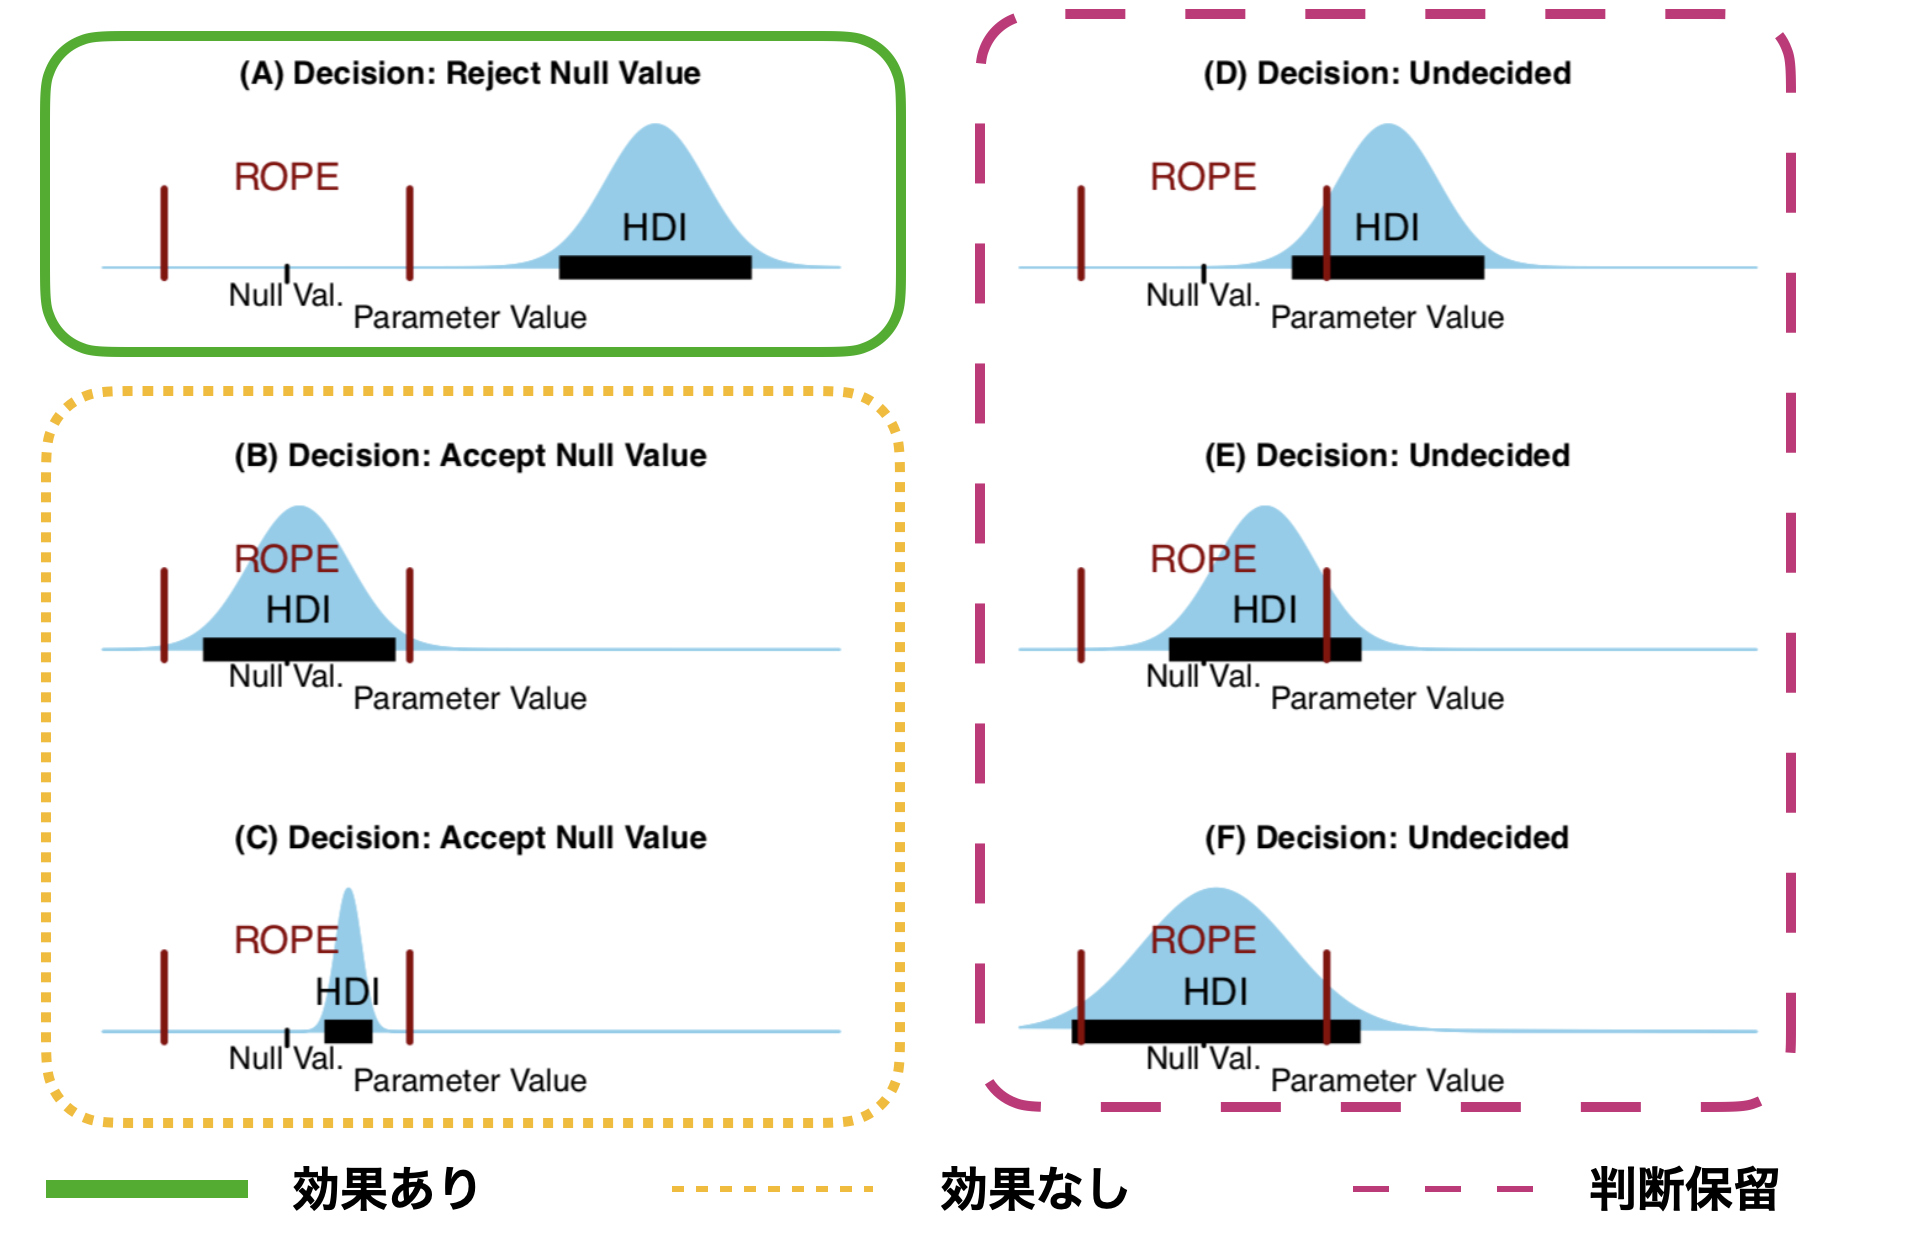
\includegraphics[keepaspectratio,width=0.8\linewidth]{../images/27_bayesian3/Krschke2018.png}
	\caption{実質的に等価な範囲による判断\parencite{kruschke2018rejecting}}
	\label{fig::27_01}
\end{figure}


During decision making, the null hypothesis test involves a confrontation between a "model competition" of null and alternative hypotheses, and a decision is made while allowing for a 5% error rate. The reason for this form is that the population mean is at one specific point, and we are searching for it, so ultimately the estimation is reduced to a binary choice of "correct or incorrect."

However, in Bayesian statistics, we don't know where the population mean is. Instead, we express our uncertainty about it in terms of probability, saying "it's probably around here". Whether there is an unknowable point or a probability distribution in the first place is a matter of philosophical debate. Regardless, instead of betting on whether it exists or not, we are actually comparing distributions. So let's just say it is somewhere in this 95% interval. The graph shows the 95% interval, and if it exists somewhere within this range, the lower 95% point of Group B is higher than the upper 95% point of Group A. As there is no overlap between the confidence intervals of these two groups, we can say that there is a significant difference between them. On the other hand, since there is an overlap in the intervals for Group A and Group C, and for Group B and Group C, we cannot say that there is a significant difference between these combinations.

This is it! That's all. For the null hypothesis test, the correct expression is "We cannot say there is no difference, and there is a 5% chance of making an error by saying so." It's still convoluted. On the other hand, the result of Bayes estimation states "There is a 95% chance that there is a difference." The term "chance" in this context refers to the strength of the claim, so it can be 50% or 99%, and 99% would have a stronger claim. Unlike the interpretation of the $p$-value for the null hypothesis test, which is not very intuitive, Bayes estimation is straightforward and easy to understand. Unlike the $p$-value, where saying that 1% is stronger than 5% is not possible because it is not a numerical value for the data or the parameters, but rather a criteria, which is established under the assumption of the null hypothesis, representing the degree of rarity of the actual value. On the other hand, the results obtained by Bayesian estimation are only the estimation range of the parameters. Therefore, it is very suitable for considering the true value from this estimation. This makes it clear that sticking to 5% is pointless.

You are a translator. 

This is not necessarily a story specific to Bayes' theorem. Using the frequentist method of moment estimation to estimate intervals, it is possible to consider whether there is a difference or not by looking at the confidence intervals. If the confidence intervals for each group are large and overlap, it is difficult to judge where the average value is likely to be. It is too early to make a judgment. If the confidence intervals are small, it is possible to check whether the judgment is correct or not. In other words, the null hypothesis testing had a problem of determining a "judgment", so the scientific research approach should not be a short-sighted one of "failure if it is an outlier", but should strive to gradually approach what is correct. As pointed out by \citet{Toyoda2009}, what is important is not the \textbf{significance}, but rather the importance.
\[ \mbox{Significance} < \mbox{Standardized Difference (Effect Size)} < \mbox{Substantive Difference} \]
In order, there is meaningfulness to the data. It is important to know how significantly different the data is in terms of standard deviation, rather than whether or not there is a significant difference in the judgment result.

However, simply contemplating whether there is a difference or not by looking at confidence intervals or credible intervals can be difficult to write in a report. Therefore, it may be a good idea to establish criteria beforehand for determining how much difference is considered significant.
The authors of \citet{kruschke2018rejecting} argue that we should determine a \keytermE{Region Of Practical Equivalence (ROPE)} before starting any analysis. They suggest that we should judge the extent to which the highest density interval of the posterior distribution falls within this ROPE (see Figure \ref{fig::27_01}). How the ROPE is determined may vary depending on the domain knowledge of the specific field to which the analysis is being applied. For example, a difference of one centimeter in the average height between men and women would be considered practically meaningless. However, a difference of one child in the total fertility rate of a woman over her lifetime would be considered a significant difference. Whether a difference of 1 cm in an optical illusion, 1 degree in a rotational angle, or 1 ms in reaction time is considered large or not depends on the units and the domain knowledge, and cannot be generalized.

The null hypothesis testing has uniformly set a standard of 5%. However, this may have caused us to overlook something crucial.

\begin{figure}[ht]
	\centering
	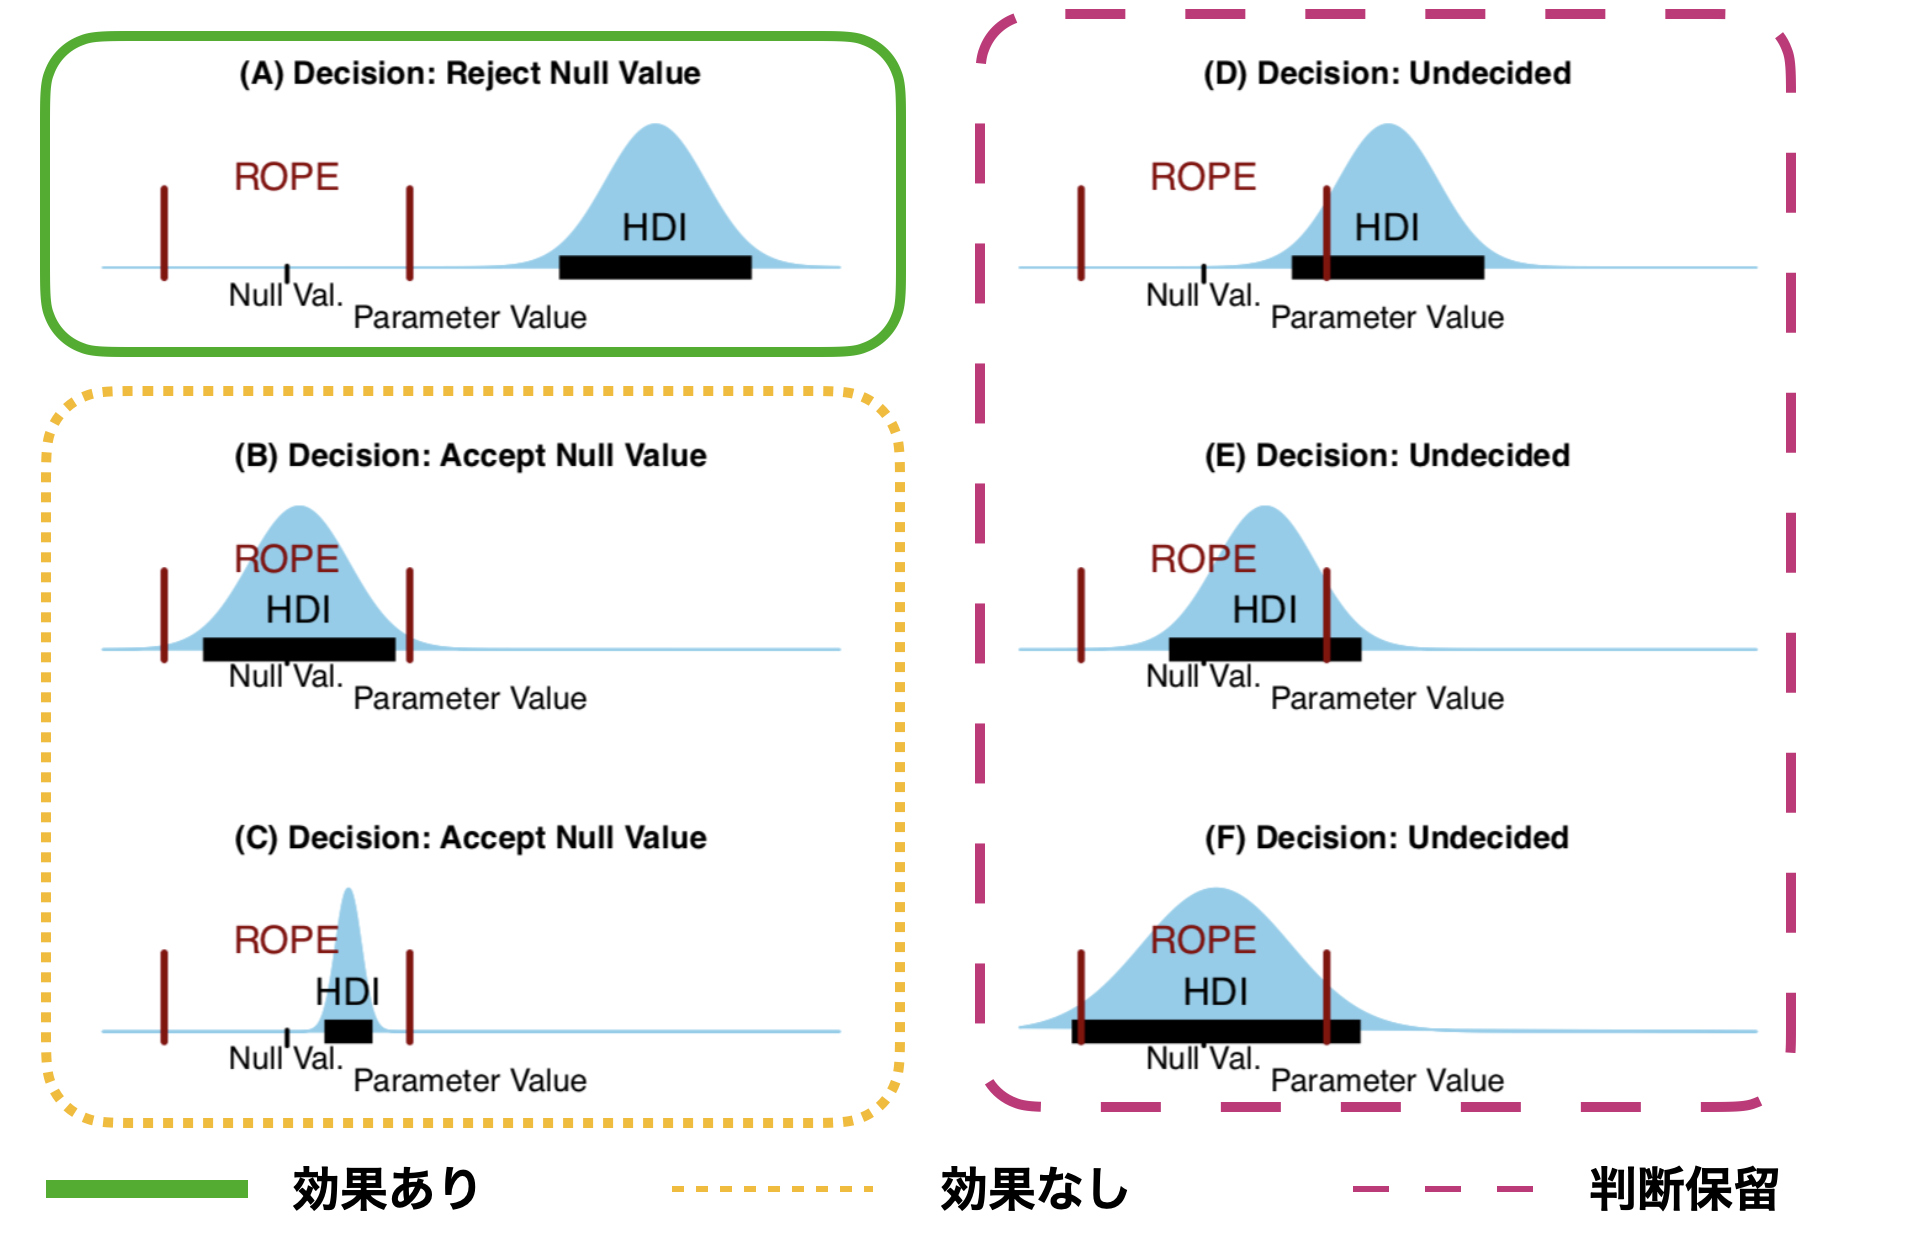
\includegraphics[keepaspectratio,width=0.8\linewidth]{../images/27_bayesian3/Krschke2018.png}
	\caption{Judgment based on substantially equivalent range \parencite{kruschke2018rejecting}}
	\label{fig::27_01}
\end{figure}


\section{Bayes Factor}
Let me introduce another perspective on criteria for decision making using Bayesian methods. This is called the \keytermE{Bayes Factor}.

Let's take another look at Bayes' formula. Bayes' formula is as follows:

\[ p(\theta\mid D) = \frac{p(D\mid \theta)p(\theta)}{p(D)} \]

In words, the posterior probability is the product of the prior probability and the likelihood, divided by the marginal likelihood.
As we have focused on the shape of the posterior distribution so far, the discussion has been centered on the prior probability and likelihood that correspond to the numerator. However, let's now direct our attention to the denominator. The denominator is $p(D)$, which represents the probability of observing the data and is a constant that we can ignore, or so we've said. However, when considering model comparison, it becomes significant.

Now, let's talk about the null hypothesis test, which is a confrontation between the model of the null hypothesis and the model of the alternative hypothesis. Let's add the condition of verifying using a model $\mathcal{M}$ to the Bayes' formula.

\[ p(\theta \mid D,\mathcal{M}) = \frac{p(D\mid \theta,\mathcal{M})p(\theta \mid \mathcal{M})}{p(D\mid \mathcal{M})} \]

All elements now have the condition "under the assumption of a certain model" added to them. Now let's focus on the denominator here. To put $p(D\mid \mathcal{M})$ into words, it represents the probability of the data given the model $\mathcal{M}$.
The model $\mathcal{M}$ is a model with parameters $\theta$, but if these parameters only have two states, for example, $\theta_1$ and $\theta_2$, then the following computation can be performed using these two states. However, the TeX code should not be modified.

\[ p(D\mid \mathcal{M}) = p(D\mid \theta_1,\mathcal{M})p(\theta_1\mid \mathcal{M}) + p(D\mid \theta_2,\mathcal{M})p(\theta_2\mid \mathcal{M}) \]

This means that we have marginalized with respect to $\theta$. When we add up all the possible patterns of probabilities, the parameter disappears. Generalizing to the case of a discrete parameter with K states, we can write it as follows.

\[ p(D\mid \mathcal{M}) = \sum_{k=1}^K p(D\mid \theta_k,\mathcal{M})p(\theta_k\mid \mathcal{M}) \]

Even with continuous parameters, the symbol for summation $\sim$ changes to the integration symbol $\int$, but the equation remains almost the same.

\[ p(D \mid \mathcal{M}) = \int p(D\mid \theta,\mathcal{M})p(\theta\mid\mathcal{M}) d\theta \]

When thinking in this way, $p(D \mid \mathcal{M})$ represents the probability of obtaining the data given the model, and its calculation is based on counting "all the probabilities assumed by the model comprehensively."
The logic of the hypothesis test involves two models, the null hypothesis model and the alternative hypothesis model. Therefore, the comparison is between the models $p(D \mid \mathcal{M}_{null})$ and $p(D \mid \mathcal{M}_{alt})$.
This probability represents the likelihood of obtaining data from the assumed model, which is to say, it also represents how well the model is supported by the data. If the expected data comes out as assumed by the model, this number will be high, whereas if data that was not expected by the model is obtained, this number will be low. If the model gives vague, wide-ranging predictions like "anything can come out," it means that the parameter range is very wide, and if data is calculated over this entire range, data is more likely to come out from places where the model did not make any predictions. In the end, this value will become small. In other words, "models that can explain everything" end up explaining nothing. Have you understood the meaning of this value representing the degree to which the model is supported by the data?

In addition, let's consider the following numbers.

\[ BF_{12} = \frac{p(D\mid \mathcal{M}_1)}{p(D\mid \mathcal{M}_2)} \]

This number is called the \keytermE{Bayes Factor}, which represents how much more the data supports Model 1 over Model 2. If this number is larger than 1.0, it means that Model 1 is relatively more strongly supported by the data than Model 2. Conversely, if it is less than 1.0, it means that Model 2 is better than Model 1. It can also be expressed as $BF_{21}$, as it is a comparison between models. If we assume that Model 1 is the alternative hypothesis and Model 2 is the null hypothesis, we can see which one better represents the data and which one is more supported by the data. However, with this approach, we can also actively support the null hypothesis that "there is no difference". When expressed as an indicator, we tend to seek a guideline for what is considered a "good" value for the BF (generally considered to be 3 or more), but we may end up with a meaningless target value similar to that of a study aiming for a 5% $p$-value. Therefore, it may be better not to think about such things.

Anyway, this is one of the methods for model comparison in the Bayesian approach. There are also methods to evaluate the predictive power of the model from the perspective of information statistical theory, using an index called WAIC\footnote{Please refer to \citet{Hamada201912} for details.}, but all of them use the marginal likelihood. The problem is that calculating the marginal likelihood is very difficult. When there are multiple parameters, it is necessary to perform a multiple integration for all combinations of all parameters in the denominator. This is very difficult in numerical calculation, making it quite challenging in practical applications.

However, when it comes to the relationship between the null hypothesis and the alternative hypothesis, there is a convenient way to calculate the Bayes factor without modifying the TeX code. For example, in the case of testing the difference between two group means, the null hypothesis is that $\mu_1=\mu_2$ and the alternative hypothesis is that $\mu_1\neq\mu_2$. The alternative hypothesis is a hypothesis that says it's ok if the two population means are not equal, in other words, $\mu_1-\mu_2 \neq 0$. If we take the difference $\mu_1-\mu_2$ as the X-axis, the null hypothesis becomes a pinpoint, partial hypothesis where $X=0$. In the broad range of the alternative hypothesis, the null hypothesis is a subset or a specific case. In cases of nested hypotheses such as this, the \keytermE{Savage-Dickey method}\citep{Lee201709} can be used to calculate the Bayes factor.

\section{Advantages of Bayesian Estimation}
I have explained a lot, but it is worth noting that Bayesian estimation can also be used to determine whether a treatment has an effect or whether there is a difference in means.
There are several methods for thinking about interval estimation, as well as using an indicator called the Bayes factor, which has advantages that were not present in null hypothesis testing. Let's list and explain three of them below.
"You can evaluate it at its actual size."
One issue is that it's easy to fall into a binary decision when dealing with 1-bit judgments, as mentioned earlier. By discussing the difference, or how much impact there was directly, one is considering the effect size from the beginning. The problem with null hypothesis testing is that there is a risk of constructing a debate with a rigid "it is significant no matter what" approach, while ignoring whether there was a large or small difference. However, if one uses Bayesian estimation, it is possible to prevent this misunderstanding in advance. 
Especially when conducting exploratory research on phenomena with multiple unknown states, hastily making decisions with null hypothesis testing can lead to hypotheses or theories being misled in the wrong direction, so this is an important point for the field of psychology as a whole. Of course, this is an expression of my "Bayesian bias", and it's still better to discuss the estimated value and its confidence interval without performing judgment, even with a frequentist perspective. If one uses maximum likelihood estimation for linear models, it is not necessary to make a judgment and only consider the confidence interval.

"Unleashed from issues of correction and multiplicity."
In t-tests and analysis of variance, we have explained the need to test if variances are equal and, if the assumption of equality is not maintained, to use Welch's correction or Greenhouse-Geisser's correction if the assumption of sphericity is violated. These are like patches applied along with the theoretical development of the original ANOVA, and they were very troublesome issues. Additionally, the results of analysis of variance require post-hoc tests. We could not say that there were no differences, so it was necessary to search again where they were present, and consider various corrections and adjustments to combat the inflation of the $\alpha$ level. This, too, was a very troublesome issue.

With Bayesian estimation, this problem can be easily solved. As for the inflation of the latter $\alpha$, it is not a problem in the first place because it does not involve setting null hypotheses or making probabilistic judgments. There is no need to pile up tests on whether the variances are equal or whether the assumption of sphericity is maintained. Simply estimating the variances and covariances as unknown parameters does not involve probabilistic judgments.

One problem inherent in hypothesis testing is the issue of \textbf{stopping rules}. For example, the research method where the data of 5 individuals was collected, analyzed, and found to be not significant, and then collected data for 10 individuals which was still not significant, followed by 20 individuals which finally yielded a significant result, is \textbf{unacceptable} according to hypothesis testing. Hypothesis testing dictates that all rules for the analysis must be established prior to collecting data and must be fair and unbiased. As sample size increases, the likelihood of a significant result also increases. Therefore, gradually increasing the sample size until a significant result is obtained is considered an unjust method, similar to extending a game until one wins. On the other hand, Bayesian methods update information as more data is added, so incorporating the information obtained from the first 5 individuals as prior information and calculating the posterior distribution from an additional 5 individuals is a natural approach.\footnote{This method, "using the posterior distribution of the first 5 individuals as prior information and calculating the posterior distribution of an additional 5 individuals," and "calculating the posterior distribution for all 10 individuals at once," will yield the same posterior distribution.} One advantage of Bayesian methods is that they can naturally avoid the problems inherent in hypothesis testing, especially those that beginners tend to inadvertently fall into. However, the problem with stopping rules, where the effort to achieve a significant result intersects with scientific judgment, is a difficult one to tackle even from a research practice and educational perspective. After all, research is a part of human activity and at times, it can be difficult to distinguish between the two. Of course, deliberately manipulating data to obtain a significant result is considered a scientific crime that is tantamount to fabrication and falsification.

"Can actively support the null hypothesis"
In practical research, there may be scenes where you want to demonstrate that there is no relationship or no effect. However, within the framework of null hypothesis testing, this cannot be done. The reason is that null hypothesis testing relies on rejecting the hypothesis, so it is impossible to verify whether the assumption of "no difference or no effect" is correct through this method of calculation.

In the process of Bayesian estimation, instead of imposing an unreasonable null hypothesis, we simply place a natural probability model, so whether the slope is zero or not can be expressed by whether it is contained in the confidence interval. As the confidence interval narrows, the confidence in that slope increases, so we can say that there is no clear difference.

I have also mentioned that null hypothesis testing involves model comparison. In Bayesian estimation, we can also compare models and express which model is more supported by the data using the Bayes factor. At this point, we can assert aggressively that the null hypothesis model with a slope of 0 is more supported by the data than other models, and claim that there is "no difference".

\subsection{Expanding into the World of Bayesian Inference}
Looking at it this way, the hypothesis testing might seem a little constricting. To arrive at the right conclusions, hypothesis testing is designed with very strict rules and manuals, but it cannot be denied that these manuals tend to be too rigid. At this point, does it not bother you that linear models are at the core of it all? So far, the only tool available was hypothesis testing, which forced research into the framework of normal distribution and linearity, due to the historical circumstances surrounding it.

For example, since data on ratios does not follow a normal distribution, it is not suitable for analysis of variance. If analysis of variance is absolutely necessary, data can be corrected by transforming it by taking the logarithm for items such as income and response time that do not follow a normal distribution, or by correcting it by transforming by taking an angle for the data. This transformation of data has been practiced throughout history as there was no other method of verification other than standardizing it for analysis of variance.

The linear model has also evolved, and in the Generalized Linear Model (GLM) which removes the assumption of normal distribution, you can select distributions that match the data generation process, such as the binomial or Poisson distribution. It should be noted that the GLM is also called the General Linear Model (GLM) in English, and it means "transforming" in Japanese, but the distinction between -ze and -se at the end of the word can result in a significant difference in meaning. Nowadays, the basic approach involves selecting an appropriate probability function or likelihood function rather than transforming the data.

However, the linear property is still retained. Some people may wonder if it is possible to express variable relationships more freely. Of course, it is possible, and the idea of \textit{modeling} non-linear models has become more and more widespread in modern psychology. Bayesian statistics is particularly powerful and helpful in estimating the parameters of these models, and this approach is commonly referred to as \textit{Bayesian modeling}.

In the future of psychology, it is expected that models and analysis methods utilizing the power of Bayes will continue to proliferate. We will discuss this in more detail during the sister lecture, Applied Data Analysis in Psychology.


\end{document}
